%% Lab Report for EEET2493_labreport_template.tex
%% V1.0
%% 2019/01/16
%% This is the template for a Lab report following an IEEE paper. Modified by Francisco Tovar after Michael Sheel original document.


%% This is a skeleton file demonstrating the use of IEEEtran.cls
%% (requires IEEEtran.cls version 1.8b or later) with an IEEE
%% journal paper.
%%
%% Support sites:
%% http://www.michaelshell.org/tex/ieeetran/
%% http://www.ctan.org/pkg/ieeetran
%% and
%% http://www.ieee.org/

%%*************************************************************************
%% Legal Notice:
%% This code is offered as-is without any warranty either expressed or
%% implied; without even the implied warranty of MERCHANTABILITY or
%% FITNESS FOR A PARTICULAR PURPOSE! 
%% User assumes all risk.
%% In no event shall the IEEE or any contributor to this code be liable for
%% any damages or losses, including, but not limited to, incidental,
%% consequential, or any other damages, resulting from the use or misuse
%% of any information contained here.
%%
%% All comments are the opinions of their respective authors and are not
%% necessarily endorsed by the IEEE.
%%
%% This work is distributed under the LaTeX Project Public License (LPPL)
%% ( http://www.latex-project.org/ ) version 1.3, and may be freely used,
%% distributed and modified. A copy of the LPPL, version 1.3, is included
%% in the base LaTeX documentation of all distributions of LaTeX released
%% 2003/12/01 or later.
%% Retain all contribution notices and credits.
%% ** Modified files should be clearly indicated as such, including  **
%% ** renaming them and changing author support contact information. **
%%*************************************************************************

\documentclass[10pt,a4paper,journal]{IEEEtran}

% *** CITATION PACKAGES ***
\usepackage[style=ieee,journaltitle=false,eventtitle=false,publisher=false,booktitle=false]{biblatex} 
\bibliography{example_bib.bib}    %your file created using JabRef

% *** MATH PACKAGES ***
\usepackage{amsmath}

% *** PDF, URL AND HYPERLINK PACKAGES ***
\usepackage{url}
% correct bad hyphenation here
\hyphenation{op-tical net-works semi-conduc-tor common subject-ed conditions}
\usepackage{graphicx}  %needed to include png, eps figures
\usepackage{float}  % used to fix location of images i.e.\begin{figure}[H]
\graphicspath{{./img/}}

% custom fonts
% \usepackage[T1]{fontenc}
% \usepackage{palatino}

% Tables 
\usepackage{amsmath}
\usepackage{multicol}
\usepackage{csquotes}
\usepackage{verbatim}
\usepackage{makecell}
\usepackage{gensymb}
\usepackage{dingbat}
\usepackage{siunitx}
\usepackage{tabularx}
\usepackage{colortbl}
\usepackage[table]{xcolor}
\usepackage[labelfont=rm]{caption}
\usepackage{subcaption}
\usepackage{booktabs}

% Bibiliography
\usepackage[style=ieee]{biblatex}
\usepackage{hyperref}
\addbibresource{references.bib}
% \ExecuteBibliographyOptions{journaltitle=false,eventtitle=false,publisher=false,booktitle=false}

\setlength{\parindent}{0.5cm}
\setlength{\parskip}{0pt}

% \renewcommand{\baselinestretch}{2.5}

\begin{document}

% paper title
\title{Reservoir Computing With \textit{in silico} Plants}

% author names 
\author{Maxime Cannoodt \\ \vspace{0.5cm}
        Supervisors: Prof.\ dr.\ ir.\ Francis wyffels, Dr.\ ir.\ Michiel Stock \\
        Counselors: Dr.\ ir.\ Olivier Pieters, Dr.\ ir.\ Tom De Swaef (ILVO)
        }% <-this % stops a space
        
% The report headers
% \markboth{EEET2493 Biomedical Instrumentation. Lab. Report 1, March 2019}%do not delete next lines
% {Shell \MakeLowercase{\textit{et al.}}: Bare Demo of IEEEtran.cls for IEEE Journals}

% make the title area
\maketitle

% in the abstract or keywords.
\begin{abstract}
We present a framework to evaluate the computational capabilities of plant physiological processes in plant models for physical reservoir computing (PRC).
PRC is a computing paradigm that enables the use of physical substrates for computation. 
Recently, the use of live plants in a PRC context was demonstrated. 
We expand upon this work \textit{in silico} using plant models for grapevine and wheat. 
In our experiments, we investigated the use of leaf temperature, transpiration rate, photosynthesis rate, light absorption, water flow, and hydraulic pressure as readout traits. 
Each of these traits displayed reservoir dynamics and correlated well with biologically relevant tasks. 
Surprisingly, our framework highlighted unusual behavior in mechanistic plant models, which the authors did not yet report.
We propose that the plant-modeling community can adapt the methods in this work to verify the behavior of plant models. 
We believe that this is just the starting point for plant reservoir computing.
If knowledge and technology can scale, there will be countless opportunities in agricultural technology.
\end{abstract}

% ORIGINAL ABSTRACT
% Physical reservoir computing (PRC) is a machine learning method that exploits physical materials to perform computations.
% Recently, the use of plants as a reservoir medium was successfully demonstrated.
% To expand on this work, we identified which plant physiological processes display computational capacity.
% We developed a framework for making a quantitative comparison of physiological reservoirs.
% The framework was then applied to mechanistic models of grapevine and common wheat from the literature.
% Our experiments evaluated the computational properties of leaf temperature, transpiration rate, photosynthesis rate, light absorption, water flow, and hydraulic pressure.
% In our experiments, each of these physiological traits displayed reservoir dynamics and correlated well with biologically relevant tasks.
% As a side effect, our framework highlighted unusual behavior in mechanistic plant models, which the authors did not yet report.
% We propose that the plant-modeling community can adapt the methods in this thesis to verify the behavior of plant models.






\renewcommand\IEEEkeywordsname{Keywords}
\begin{IEEEkeywords}
Physical Reservoir Computing (PRC), Unconventional Computing, Plant Physiology, functional-structural plant models (FSPMs).
\end{IEEEkeywords}


\section{Introduction}

% What is reservoir computing?
\IEEEPARstart{R}{eservoir} computing (RC) is a holistic machine learning technique commonly used with time series data.
RC is based on the emergent computational properties of nonlinear dynamical systems, the so-called reservoir.
The key to understanding reservoir computing is that all non-linearity and memory required to solve a problem are already present in the (observable) reservoir dynamics.
These dynamics are combined using a simple linear readout function to obtain the output value for a certain task.
% This simplicity makes RC a compelling alternative to deep learning techniques that require large amounts of data and computational resources to train.
RC was first introduced as an alternative to trained recurrent neural networks and as a more biologically plausible computing model
% \cite{jaeger_echo_2002}. 
\cite{jaeger_echo_2002, maass_real-time_2002, steil_backpropagation-decorrelation_2004}. 
Later it was observed that two key features of said novel ideas: combining non-linearity and memory, can be identified in many physical systems as well, and there exists a rich literature on the use of physical media as computational resources \cite{tanaka_recent_2019}, giving rise the physical reservoir computing (PRC). Here, the reservoir state is partially inferred from sensor data observing the dynamical system from different spatial positions \cite{burms_reward-modulated_2015}, as illustrated in \mbox{Figure~\ref{fig:prc_examples}}.


\begin{figure}[t]
	\centering
    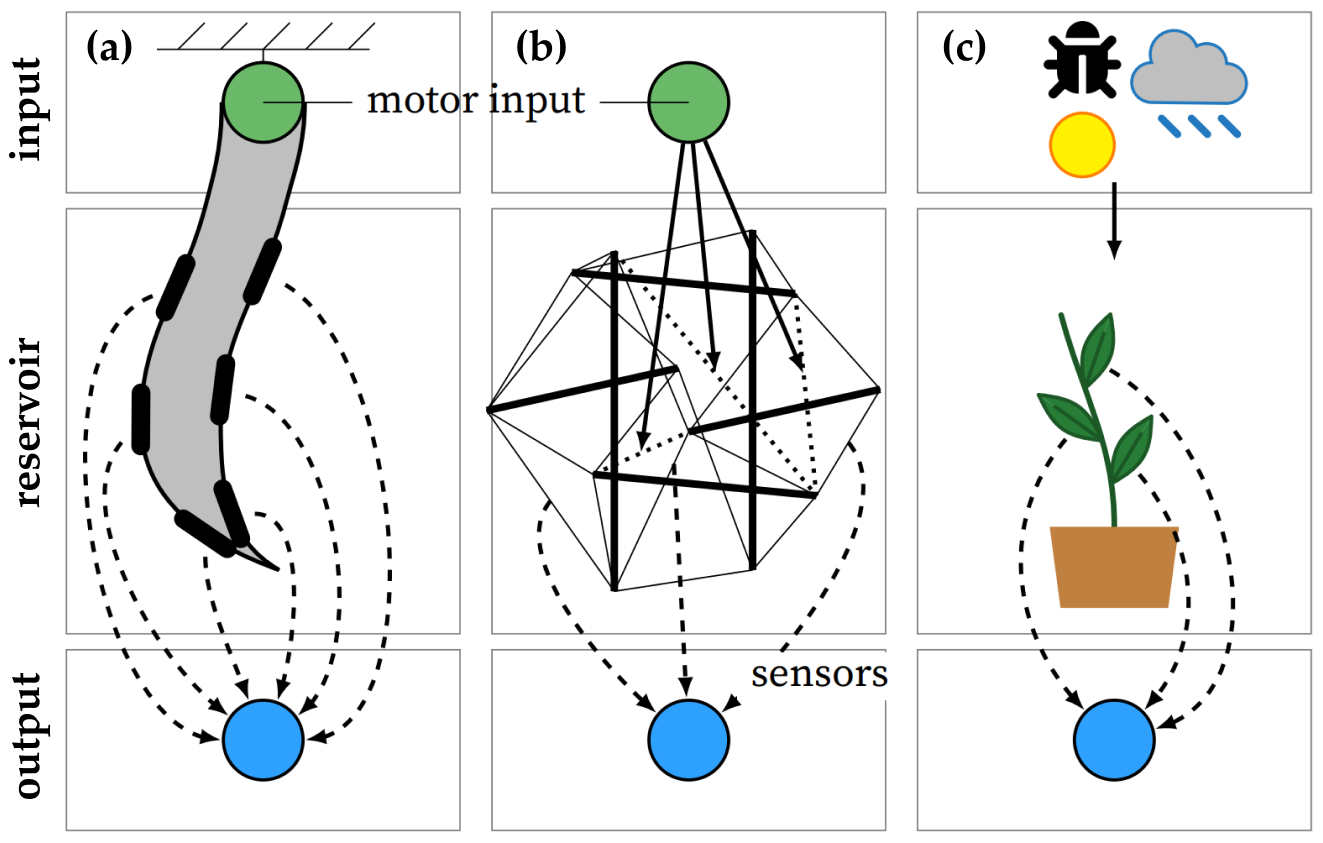
\includegraphics[width=\linewidth]{imgs/prc-illustration-small.png}
	\caption{\small Illustration of different physical reservoir computing implementations.
	            (a) Bioinspired silicone arm with integrated deformation sensors \cite{nakajima_information_2015}.
	            (b) Tensegrity robot made of beams and springs \cite{caluwaerts_locomotion_2013}. Force sensors measure the dynamics of the spring-mass system.
	            (c) The plant physiological reservoir proposed in this work.
    	 	Illustration from Pieters (2022)\supercite{pieters_reservoir_2022} with permission from the author.}
	\label{fig:prc_examples}
\end{figure}


% What is reservoir computing with plants?
Plants can also be interpreted as a computational resource.
The plant's environment is its input, and its health, growth, and behavior result from processing this information.
Interpreting plants as information-processing organisms is not a new idea.
A large body of research indicates that plants observe their environment, have memory, and are capable of learning complex patterns \cite{mancuso_revolutionary_2018}. 
Experiments by Adamatzky et al. have shown limited yet promising success in exploiting plant intelligence to implement various functions and algorithms \cite{stepney_computers_2018}.
Their work serves as experimental evidence that plants can compute highly nonlinear functions.
Most recently, Pieters demonstrated the first successful application of reservoir computing with plants \cite{pieters_reservoir_2022}. 
His research shows that \textit{Fragaria × ananassa} (strawberry) is capable of performing several environmental, eco-physiological, and computational tasks, paving the way to apply reservoir computing more broadly to a variety of crops.


% Outline of my research contribution
The work by Pieters has shown that reservoir computing with plants is possible.
Now, a more thorough examination of the reservoir dynamics of plant physiological processes is warranted.
In this work, we further investigated the reservoir dynamics present in plants.
% Why in silico plants?
We conducted our research with computer simulations of plants.
Working with simulations provided the freedom to observe the plant's physiological processes without the need for sensing technology or laboratory setups.
It gives us a first intuition into which processes show promising reservoir dynamics, which informs future research with \textit{in vivo} specimens.
% RC can also contribute to FSPM development by identifying flaws in physiological models that previously went unnoticed.

% \section{Related Work}


\section{Materials and Methods}

\subsection{Experimental Design}

To perform useful computations, a reservoir must show input separation with regard to the relevant tasks and fading memory of past environmental conditions \cite{nakajima_information_2015}.
We investigated linear task separation and memory capacity in several observable eco-physiological processes by performing relevant environmental and eco-physiological reservoir tasks. 
% These experiments identified a set of promising physiological reservoirs for future RC research.
We also verified whether these physiological processes displayed the fading memory property, an essential precondition for performing deterministic computations.
We propose an experimental framework for quantitatively measuring these properties in plant physiological processes.
The results from these experiments highlight which physiological reservoirs to pursue in future RC research.

\subsubsection{Input Separation}

% Experiment details
The reservoir readout is a strictly linear function of the observed reservoir state. 
So, to perform nonlinear computation, the reservoir must transform its inputs such that the desired task becomes a linear function of the reservoir observations.
To measure the input separation with regard to biologically relevant tasks, we used three categories of targets, previously established by Pieters: (i) predicting current environmental conditions, (ii) predicting the plant's eco-physiological performance, and (iii) computational benchmarks.
Predicting environmental inputs gives us a first indication of the plant's coupling with the environment.
Next, eco-physiological tasks indicate whether the observed reservoir is effective at solving biological problems.
Finally, computational benchmarks can measure the reservoir's degree of nonlinearity and memory.
We used three benchmarks: a delay line to measure memory capacity, a polynomial expansion to measure nonlinearity, and the Nonlinear Autoregressive Moving Average (NARMA) benchmark, a common benchmark for RC \cite{nakajima_information_2015}. 
The NARMA system is defined as:
\begin{equation} \label{eq:narma}
\begin{split}
    y(t+1) & = \alpha y(t) + \beta y(t) \left[ \sum_{i=0}^{n-1} y(t-i) \right] \\ 
    & + \gamma x(t-n+1) x(t) + \delta
\end{split}
\end{equation}
where $n$ tunes the nonlinearity and memory of the task and the parameters $\alpha$, $\beta$, $\gamma$, and $\delta$ are set to 0.3, 0.05, 1.5 and 0.1 \cite{nakajima_information_2015}.
Each computational task uses an environmental input as base signal.

% Performance metric
We measured the prediction accuracy of each physiological reservoir for a given task using the normalized mean square error (NMSE) metric:
\begin{equation} \label{eq:nmse}
\text{NMSE} = \frac{1}{N} \sum_{t=1}^{N} \frac{\left(y[t] - \hat{y}[t]\right)^{2}}{\text{var}(y)} 
\end{equation}
A lower score means a more accurate prediction.
The NMSE has several advantages over regular mean square error \cite{pieters_reservoir_2022}.
Because it is normalized, the results can be compared between reservoir-task pairings, including between plants.
It is also easy to interpret: a perfect predictor scores 0.0, while predicting the signal mean for every step yields a score of 1.0.


\subsubsection{Fading Memory}

% Experiment description
To perform reliable computations, a reservoir must display the same behavior whenever it is subjected to the same input sequence \cite{nakajima_physical_2020}.
In practice, this means past inputs should have a fading influence over the reservoir's present state \cite{lukosevicius_reservoir_2012}.
The period over which this influence fades forms a trade-off between short-term accuracy and long-term memory.
To test fading memory in physiological processes, we designed an experiment in which an impulse is applied to the plant for a brief period, as illustrated in \mbox{Figure \ref{fig:methods-impulse}}.
We then compared the trajectory of the physiological reservoir with that of a control experiment that did not receive the impulse. 
The impulse can be applied to any of the environmental inputs.
The amplitude and duration of the impulse should remain within realistic boundaries so that an actual plant would not suffer permanent damage that alters the reservoir dynamics.

% Performance metric.
To quantify the divergence $\delta(t)$ between two reservoir trajectories at a given time step, we used a modified NMSE metric:
\begin{equation} \label{eq:divergence}
    \delta(t) = \frac{1}{p} \sum_{i=1}^{p} \frac{\left( \mathbf{X}_i^{C}(t) - \mathbf{X}_i^{E}(t) \right)^{2}}{\text{var}\left( \mathbf{X}_i^{C} \right)}
\end{equation}
where $p$ is the size of the observed reservoir, $\mathbf{X}^{C}$ the reservoir state in the control experiment, and $\mathbf{X}^{E}$ the reservoir state during the impulse experiment.
A reservoir affected by the impulse will show a peak in divergence from the control experiment once the impulse is applied.
If the physiological process displays fading memory, the divergence should go down to pre-impulse levels in a finite amount of time after the artificial stimulus is removed. 

\begin{figure}[t]
	\centering
    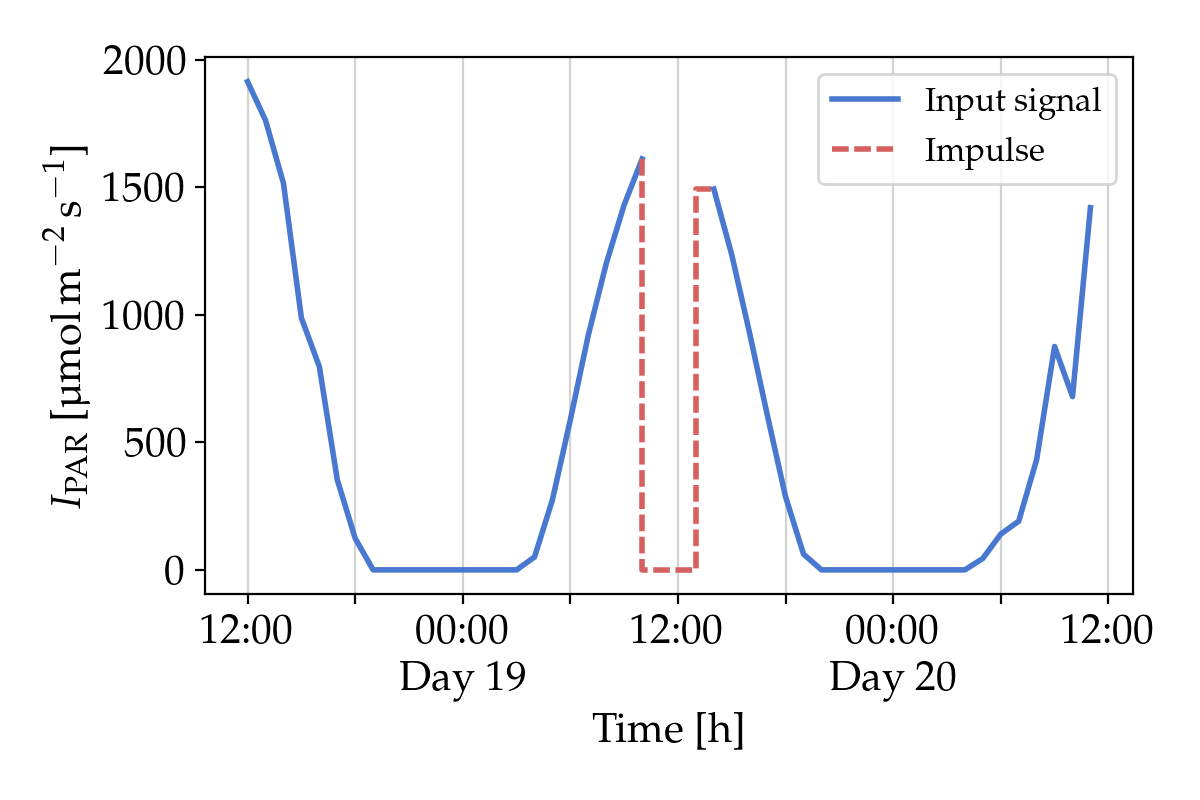
\includegraphics[width=0.93\linewidth]{imgs/cn_impulse.png}
    \vspace{-0.25cm}
	\caption{\small Applying an impulse of \SI{3}{\hour} and a value of \SI{0}{\micro\mole\per\square\meter\per\second} to the incident PAR of CN-Wheat.}
	\label{fig:methods-impulse}
\end{figure}

\subsection{Selected Plant Models}

% What are FSPMs?
We used functional-structural plant models (FSPMs) to test the experimental framework.
FSPMs represent the plant as a 3D structure of interconnected elements.
Each structural element simulates physiological processes such as photosynthesis, transpiration, and water and carbon flow \cite{coussement_turgor-driven_2020}.
This type of model has become the state-of-the-art in plant modeling in the past decade \cite{louarn_two_2020}.
% In a real paper, this could use a bit more explanation.

We present results from two FSPMs: HydroShoot \cite{albasha_hydroshoot_2019} and CN-Wheat \cite{barillot_cn-wheat_2016}.
% CHAPTER 5: HYDROSHOOT
HydroShoot is an FSPM of common grapevine.
It was published by Albasha et al. as a study of gas exchange in large plant canopies under water deficit conditions and to compare the effectiveness of different canopy shapes.
% It is based on OpenAlea, an open-source platform for plant modeling \cite{pradal_openalea_2015}.
% CHAPTER 5: CN-WHEAT
CN-Wheat, on the other hand, is a mechanistic model of common wheat developed by Barillot et al.
The model was made to simulate the effect of fertilization regimes on carbon (C) and nitrogen (N) metabolism in wheat culms during the post-flowering stages of development.
\mbox{Table \ref{table:simulation_details}} compares the model specifications for the discussed models.

% Reconciling dynamic reservoirs with the static reservoir assumption
In addition to input separation and fading memory, the PRC framework assumes the reservoir dynamics are unchanging over time.
Plants are not static reservoirs in the general case because they go through several growth phases that drastically change their structure and behavior.
Because of this, we specifically selected plant models with a static plant structure or a dynamic structure in a stage of post-vegetative growth.
For \textit{in vivo} scenarios, stationarity can be approximated by investigating reservoir dynamics within a time window for which the growth rate is negligible \cite{pieters_reservoir_2022}.

\begin{table}[b]
    \raggedright
    \caption{\small Comparison of HydroShoot and CN-Wheat: simulation details.}
    \label{table:simulation_details}
    \def\arraystretch{1.2}
    \begin{tabularx}{\linewidth}{
        >{\raggedright\arraybackslash} X
        >{\centering\arraybackslash} X
        >{\centering\arraybackslash} X
    }
        \toprule
        \textbf{} & \textbf{HydroShoot} & \textbf{CN-Wheat} \\ 
        \midrule
        \textbf{Simulation step} & \SI{1}{h} & \SI{1}{h} \\
        \arrayrulecolor{black!10!white}
        \midrule
        \textbf{Simulation duration} & 7 days & 50 days \\
        \midrule
        \textbf{Model structure} & static (idealized reservoir) & Post-vegetative growth \\
        \midrule
        \textbf{Model size} &  $\approx 10^3$ elements & 15 elements \\
        \arrayrulecolor{black}
        \bottomrule
    \end{tabularx}
\end{table}

\subsection{Considered Physiological Reservoirs}

Many physiological processes inside the plant can be considered a potential reservoir.
We limited ourselves to processes that are observable using existing, non-destructive sensing technologies.
The observable physiological processes for HydroShoot and CN-Wheat are presented in \mbox{Table \ref{table:simulation_reservoirs}}.
We had a preference for processes that are observable using image-based sensors because contactless sensors do not influence the reservoir dynamics \cite{pieters_reservoir_2022}.
Also, contactless sensing technologies may one day be the key to scaling plant RC to larger arrays of plants.
Finally, we did not consider processes that violate fading memory.

\begin{table*}[t]
    \centering
    \caption{\small Comparison of HydroShoot and CN-Wheat: physiological processes observable in each structural element. Not all are shown in the table; we only present the processes that are experimentally observable and that do not violate fading memory. Check marks indicate whether the physiological process is modeled by the FSPM.}
    \label{table:simulation_reservoirs}
    \def\arraystretch{1}
    \small
    \begin{tabularx}{0.8\linewidth}{
        >{\centering\arraybackslash} c
        >{\raggedright\arraybackslash} X
        >{\centering\arraybackslash} c
        >{\centering\arraybackslash} c
        >{\centering\arraybackslash} c
    }
        \toprule
        \textbf{Symbol} & \textbf{Description} & \textbf{Unit} & \textbf{HydroShoot} & \textbf{CN-Wheat} \\ 
        \midrule
        \(A_n\) & Net photosynthesis rate & \unit{\micro\mol\per\meter\squared\per\second} & \checkmark & \checkmark \\
        \arrayrulecolor{black!10!white}
        \midrule
        \(T_s\) & Surface temperature & \unit{\celsius} & \checkmark & \checkmark \\
        \midrule
        \(g_s\) & Stomatal conductance & \unit{\mol\per\meter\squared\per\second} & \checkmark & \checkmark \\
        \midrule
        \(E\) & Transpiration rate & \unit{\mol\of{H\textsubscript{2}O}\per\meter\squared\per\second} & \checkmark & \checkmark \\
        \midrule
        \(F\) & Water flow across segment & \unit{\kilo\gram\per\second} & \checkmark &  \\
        \midrule
        \(\Psi\) & Mean water potential of segment & \unit{\mega\pascal} & \checkmark &  \\
        \arrayrulecolor{black}
        \bottomrule
    \end{tabularx}
\end{table*}

\subsection{Reservoir Readout Model}

For the reservoir readout function we used a simple linear regression model with a bias term:
\begin{equation} \label{eq:readout}
\hat{y}[t] = w_0 + \sum_{i=1}^{p} w_i x_i[t]
\end{equation}
Where $\hat{y}$ is the predicted value, $x_{i}$ the reservoir measurements, and $w_i$ the model parameters.
To train the model parameters, we used a gradient descent algorithm to minimize the ridge regularization loss:
\begin{equation} \label{eq:l2-regularization}
    L_{\text{ridge}} = \frac{1}{N} \sum_{i=0}^{N-1} \left(y[i] - \hat{y}[i] \right)^2 + \lambda \sum_{i=1}^{p} |w_i|^2
\end{equation}
where $\lambda$ is a regularization parameter that prevents overfitting.
To find the optimal \(\lambda\), we used a parameter sweep with logarithmic spacing and a leave-one-out cross-validation scheme.
We dedicated 50\% of the experimental data for training and cross-validation and the other 50\% for testing the final model on unseen data.


% - Ridge regression model

% - Machine learning model used.
% - Training method and preprocessing used.


\section{Results and Discussion}

\subsection{Environmental and Physiological Tasks}

% Setup
We considered air temperature ($T_{\text{air}}$), relative humidity (RH) and incident photosynthetically active radiation (PAR) for the environmental targets.
% We chose these targets because of their physiological relevance and to compare the results with those already obtained for strawberry plants in \citet{pieters_reservoir_2022}.
For the physiological targets we used transpiration rate ($E$), absorbed PAR ($\Phi_{\text{PAR}}$) and net photosynthesis rate ($A_n$). 
The physiological target $A_n$ was only available for HydroShoot, while both models offer it as a physiological reservoir.

% NMSE scores
Figure \ref{fig:result-regression-scores} showcases the performance of each physiological reservoir as boxplots.
For the HydroShoot model, we observe that each reservoir performs roughly the same for a given target.
In CN-Wheat, the difference between the reservoirs is more outspoken.
For example, RH correlates relatively well with $E$ in CN-Wheat, where none of the processes in HydroShoot correlate well with RH.
We must also note that CN-Wheat significantly outperforms HydroShoot in most tasks.

% prediction accuracy
We study the time series prediction accuracy more closely in \mbox{Figure \ref{fig:result-regression-accuracy}}.
In this figure, we see that the $E$ reservoir captures the broad dynamics of $\Phi_{\text{PAR}}$ for both HydroShoot and CN-Wheat.
However, HydroShoot cannot reproduce finer details, underpredicting the highest targets and overpredicting the lowest.
Moreover, HydroShoot's predictions sometimes lag behind the target (\mbox{Figure \ref{fig:result-regression-accuracy}}, samples A and C), and other times lead the target (\mbox{Figure \ref{fig:result-regression-accuracy}}, sample D).
In contrast, CN-Wheat's transpiration rate captures finer details much better.

\subsection{Computational Benchmarks}

We based the computational benchmarks on two different input signals ($T_\text{air}$ and PAR).
For each benchmark, we compared the reservoir's advantage (or disadvantage) over a linear model of the input signal as we increased the benchmark's difficulty.
In what follows, we discuss the results for the surface temperature ($T_s$) and transpiration rate ($E$) reservoirs specifically.

% Delay line
Figure \ref{fig:result-delay-scores} shows the results for the delay line benchmark.
Both reservoirs display memory capacity for this task.
The memory for predicting the $T_\text{air}$ input can be explained by thermal inertia; the difference in heat capacity between air and the plant's water mass results in a slowed reaction to changes in ambient temperature.
The readout function can exploit this inertia to learn about past inputs.
This is only a first-order interpretation, as it does not consider e.g.\ heat lost in evaporation.
Similarly, thermal inertia can explain the results for incident solar radiation.

% Polynomial
Next, \mbox{Figure \ref{fig:result-polynomial-scores}} presents the accuracy predicting a polynomial expansion.
A polynomial relationship exists between air temperature and respiration rate, as the prediction error reaches a minimum for a degree of five.
For the other input-reservoir pairings, we see a similar performance characteristic as the linear model plus a bias penalty induced by the noisy input-reservoir relation.

% NARMA
Finally, we consider the NARMA benchmark.
In \mbox{Figure \ref{fig:result-narma-scores}} we increased the $n$ parameter from 2 up to 24. 
For the benchmark based on air temperature, only surface temperature $T_s$ outperformed the linear model. 
The same thermal inertia theory from before can explain the correlation with this NARMA benchmark.
Both $T_s$ and transpiration rate $E$ outperform the linear model for the benchmark based on incident PAR, particularly for $n$ values 8, 12, and 18.
The task becomes easier for $n$ equal to 18 and 24.
This is because of the averaging effect of Equation \ref{eq:narma} as the summation window extends over (nearly) the entire diurnal period of \SI{24}{\hour}.
\mbox{Figure \ref{fig:result-narma-accuracy}} shows the time series prediction for the NARMA8 task based on incident PAR, as predicted by surface temperature $T_s$.

\subsection{Fading Memory} \label{sec:results-fading-memory}

% Setup
\mbox{Figure \ref{fig:results-impulse-experiment}} show the divergence $\delta(t)$ (Equation \ref{eq:divergence}) in the physiological reservoirs caused by impulses of \SI{5}{\hour}. 
We applied the impulses to incident PAR with zero and high amplitudes. 
We used a value of approx.\ two times the natural maximum signal strength for the high amplitude.

\begin{figure}[t]
	\centering
    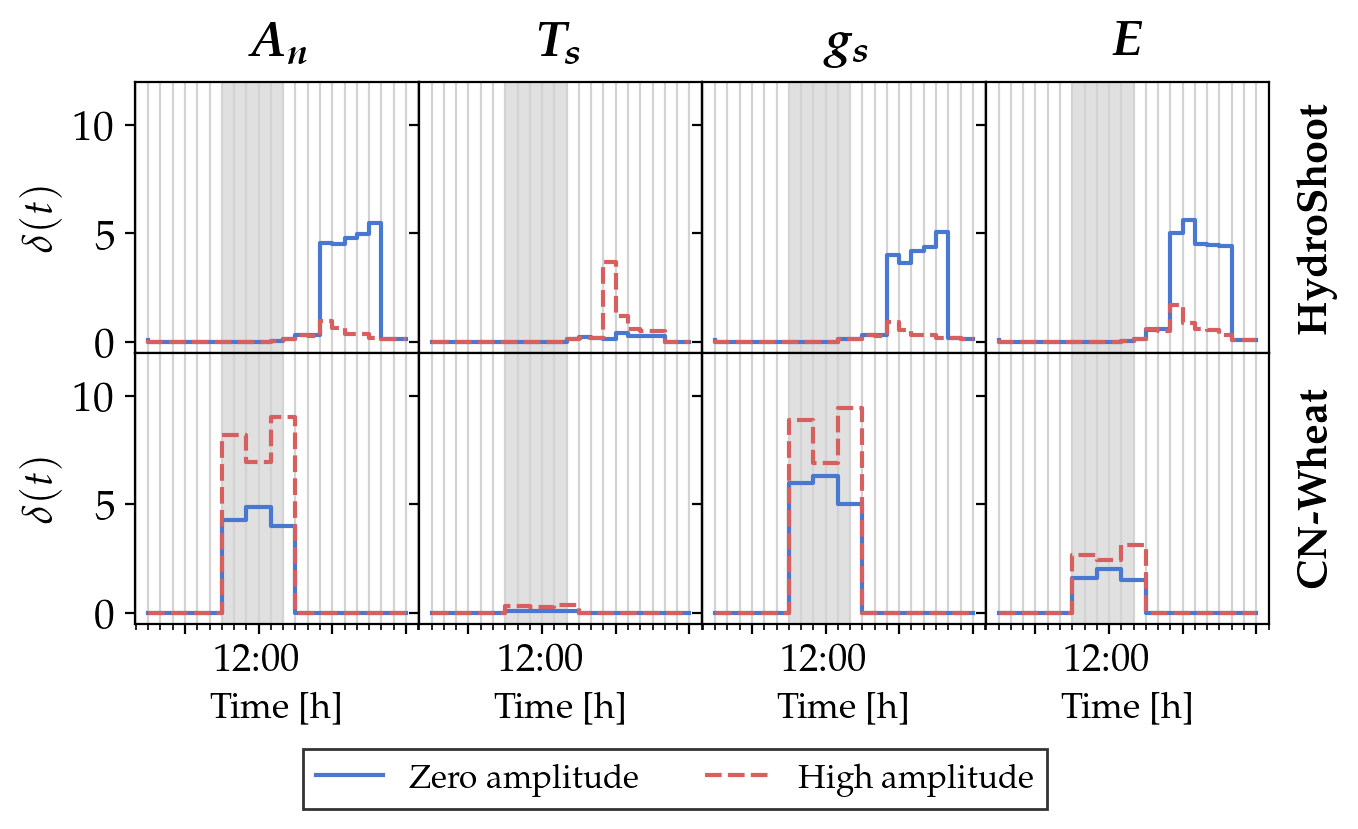
\includegraphics[width=\linewidth]{imgs/impulse_reservoirs_compact.png}
	\caption{\small 
	Predicting a time-delayed signal of $T_{\text{air}}$ and PAR using surface temperature ($T_s$) and transpiration rate ($E$).
    The reservoirs' performance is compared to a linear model that uses the benchmark's input as the only feature.
    The error bars show the scores' standard deviation.
    }
	\label{fig:results-impulse-experiment}
\end{figure}


% HydroShoot
For HydroShoot, the data shows that the reservoir divergence caused by the impulse lasts for the same duration as the impulse itself. 
However, the reservoir reacts at an \SI{8}{\hour} delay.
% HydroShoot: Delays
Investigating the experimental data revealed a continuously shifting misalignment between the diurnal cycle of the input signal and the oscillations in the physiological dynamics.
In an extreme case, the peak in transpiration rate lagged nearly a half-period behind the incident PAR.
% HydroShoot: Chaos
In addition, The data indicates that the reservoir dynamics diverge slightly during the daytime, even between plants subjected to identical conditions.
This indicates that the observed physiological processes display somewhat chaotic dynamics during daytime hours.
The chaotic behavior may be a result of numerical instabilities in the simulation.
However, there exist reports of chaotic behavior in plant physiological responses to light in the literature \cite{shabala_observations_1997}.
% HydroShoot: conclusion
The shifting delay in reservoir response is the most likely explanation for the delayed response to the artificial stimulus.
We must also attribute the slight disturbance that precedes the peak in divergence to the natural chaotic behavior.
After accounting for these two factors, no lasting memory effects are visible at the simulation scale of \SI{1}{\hour}; if there are any transient dynamics, they must occur over a much shorter time frame.


% CN-Wheat
The results for CN-Wheat reveal that the simulations responsible for our physiological reservoir update at a \SI{2}{\hour} interval, as described in the model's follow-up paper \cite{barillot_cn-wheat_2016-1}. 
Looking past the misalignment caused by the \SI{2}{\hour} simulation step, we see that the reservoir divergence disappears immediately when the real input signal resumes.
The most likely explanation is that the transient behavior lasts less than two hours, such that the coarse simulation steps mask any memory effects.

% use for conclusion to hydroshoot
These initial results imply that each considered reservoir has fading memory of incident PAR that lasts less than two hours.
Regardless, we can conclude that all reservoirs show stationary behavior w.r.t. this abiotic input.


\subsection{Potential Weaknesses}

% Correlation and bias
We used the same measurements for the reservoir as are used by the model to compute the physiological regression tasks.
This introduced positive bias into the correlation between the reservoir and the physiological targets.
This bias is especially pronounced in the accuracy of CN-Wheat for predicting total transpiration rate and absorbed PAR; 
CN-Wheat achieves near-perfect accuracy for these tasks.
To reduce this bias, we could have introduced some signal noise to the observations to make them less precise.
However, it is difficult to determine what amount of noise is appropriate in this case.


% FSPMs as weak link
Another weakness is the trust in the accuracy of the FSPMs.
Plant models are generally not verified as one hundred percent accurate copies of their real-world counterparts.
As we described in Section \ref{sec:results-fading-memory}, the HydroShoot model displayed unexpected behavior that was not reported in the original paper.
To emphasize that our results characterize the behavior of plant models, we used the names of the FSPMs instead of the plant genus. 

% Time resoultion as weak point
Finally, the lack of time resolution in the plant simulations leaves us with a weak take-away about transient memory dynamics in the studied plant species.
Though we can conclude that the considered physiological reservoirs show stationary behavior at the hour scale, we cannot state the exact duration during which past inputs influence the present reservoir dynamics.


\begin{figure*}[t]
    \centering
    \begin{subfigure}[a]{0.513\linewidth}
        \centering
        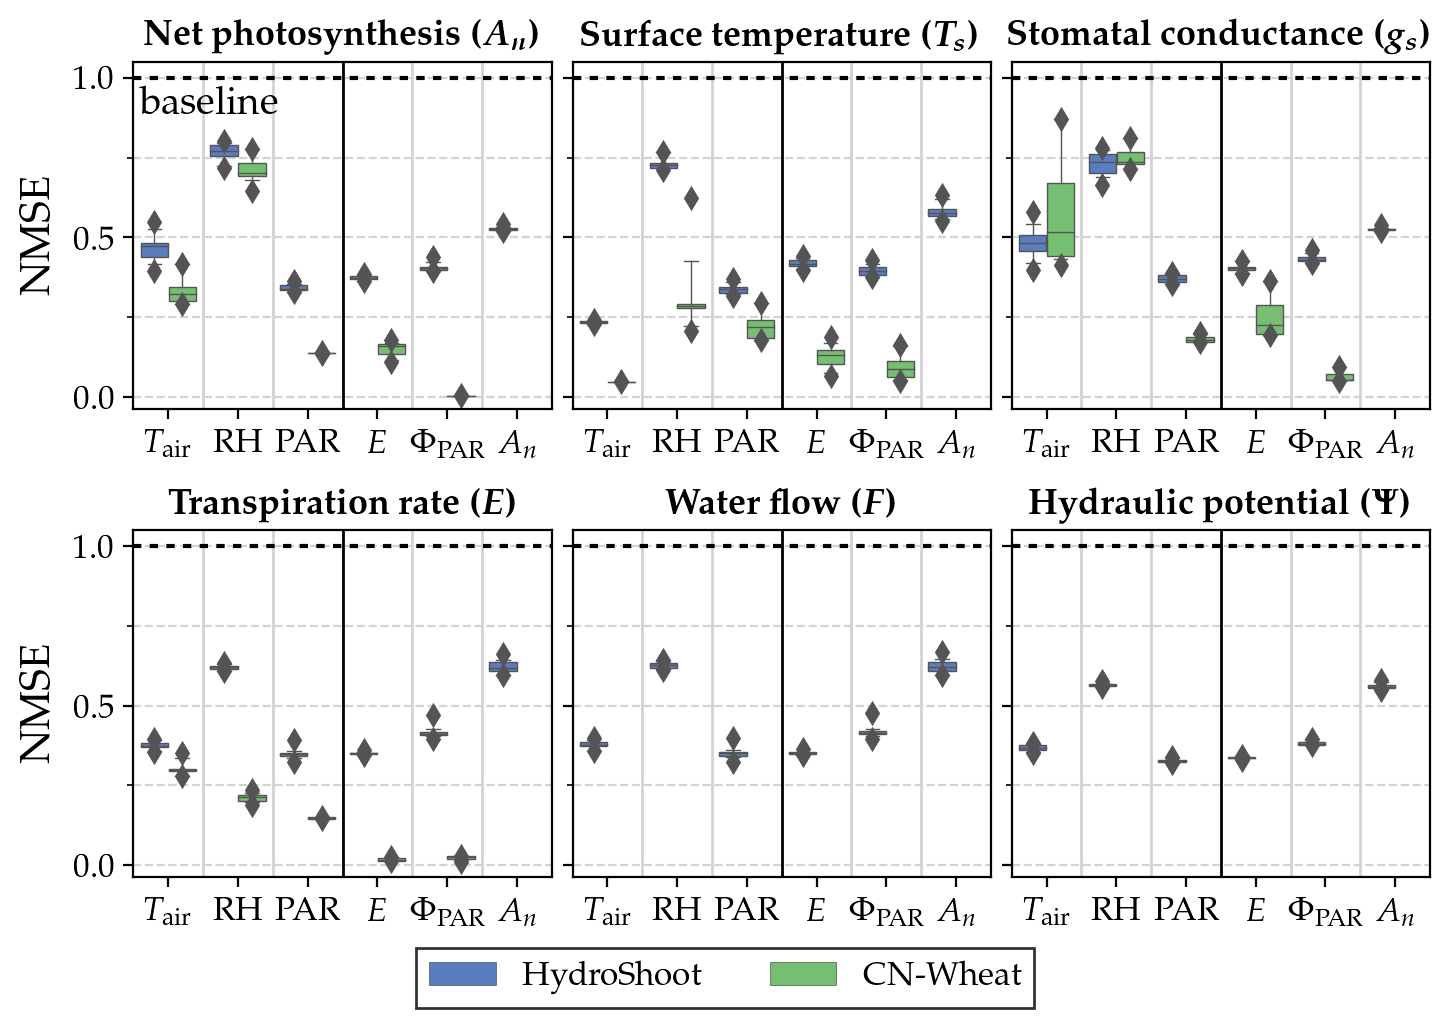
\includegraphics[width=\linewidth,height=\linewidth,keepaspectratio]{imgs/regression_res_perf_compact.png}
        \caption{\null}
        \label{fig:result-regression-scores}
    \end{subfigure}
    \hfill
    \begin{subfigure}[a]{0.427\linewidth}
        \centering
        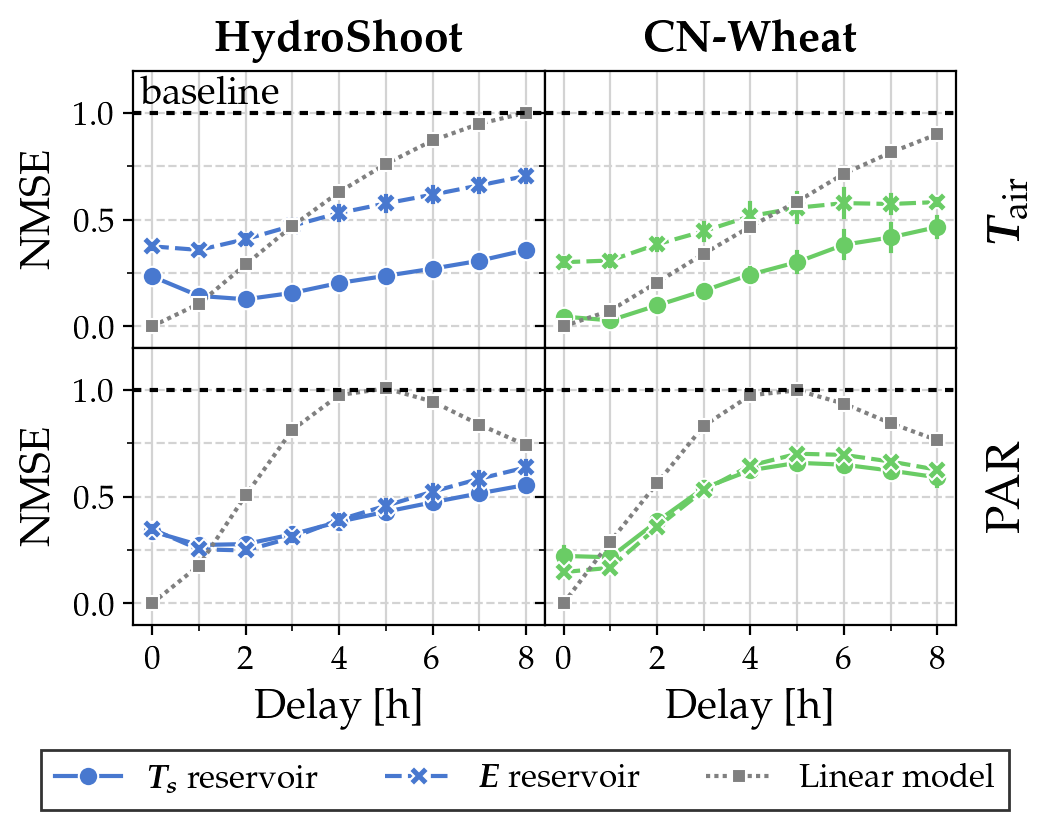
\includegraphics[width=\linewidth,height=\linewidth,keepaspectratio]{imgs/comp_delay_perf_compact.png}
        \caption{\null}
        \label{fig:result-delay-scores}
    \end{subfigure}
    \vskip\baselineskip
    \begin{subfigure}[a]{0.513\linewidth}
        \centering
        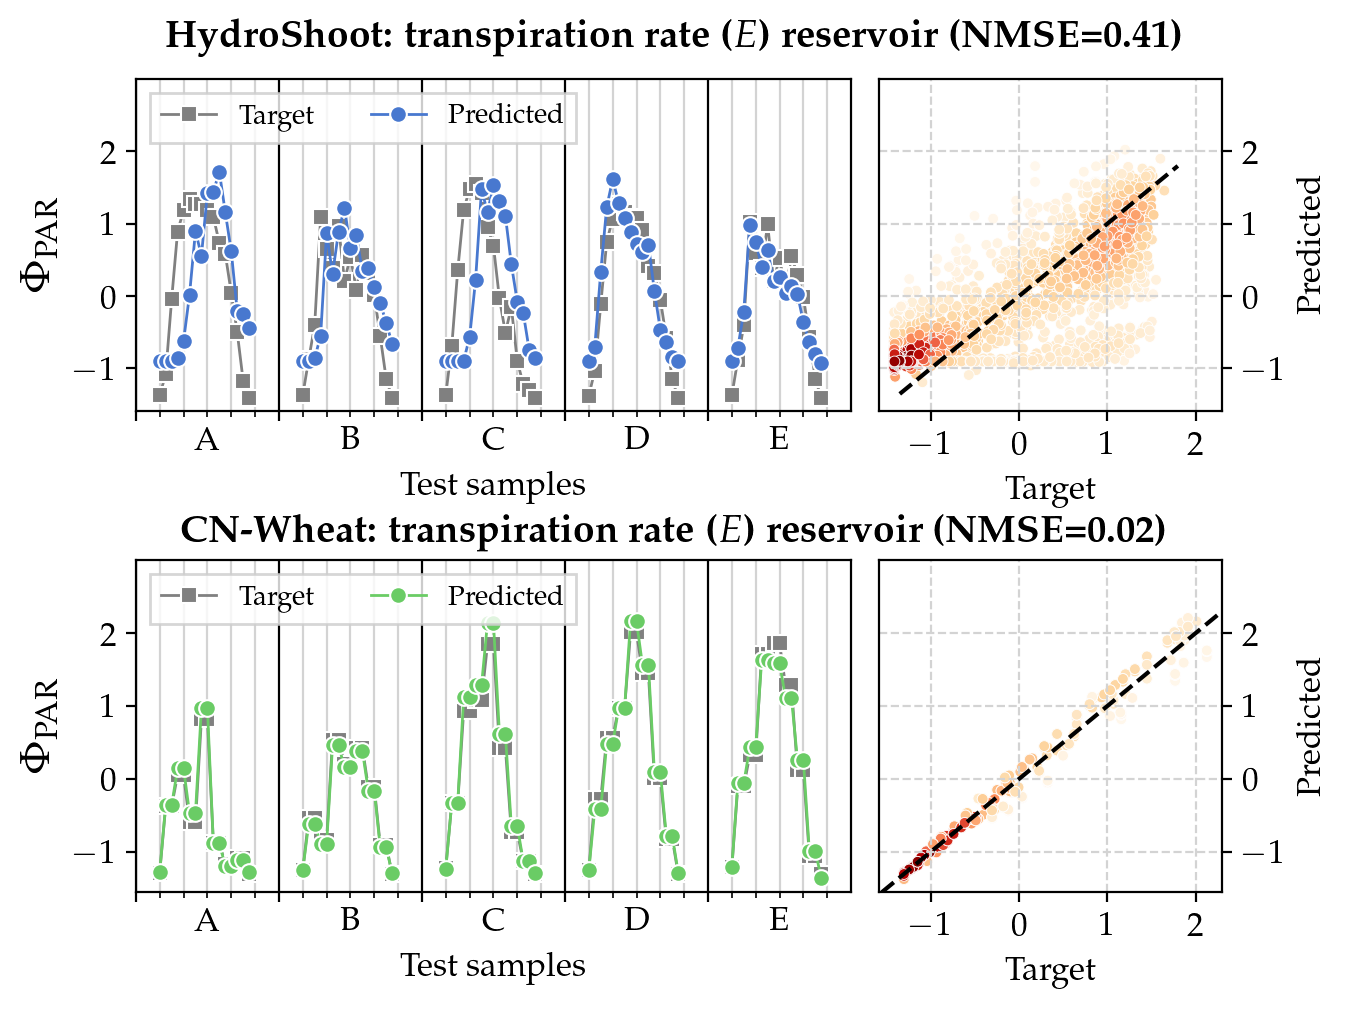
\includegraphics[width=\linewidth,height=\linewidth,keepaspectratio]{imgs/regression_res_prediction__output__custom__PARa__state__Tr_compact.png}
        \caption{\null}
        \label{fig:result-regression-accuracy}
    \end{subfigure}
    \hfill
    \begin{subfigure}[a]{0.427\linewidth}
        \centering
        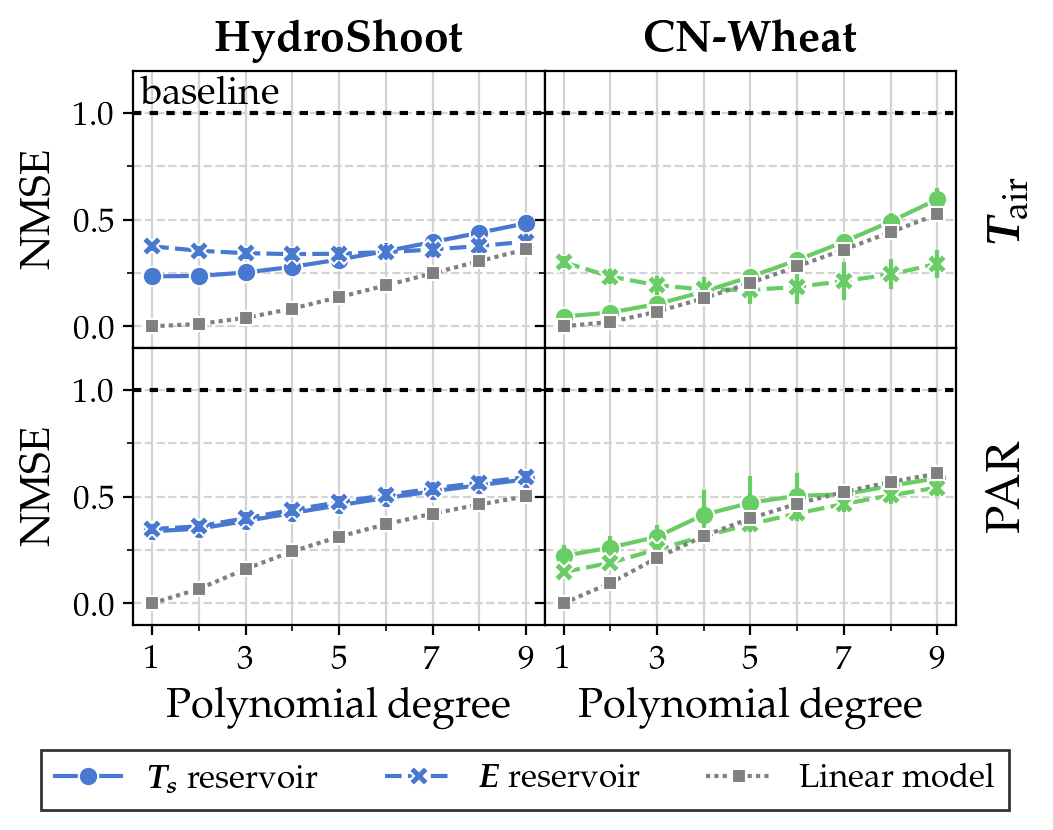
\includegraphics[width=\linewidth,height=\linewidth,keepaspectratio]{imgs/comp_polynomial_perf_compact.png}
        \caption{\null}
        \label{fig:result-polynomial-scores}
    \end{subfigure}
    \vskip\baselineskip
    \begin{subfigure}[a]{0.513\linewidth}
        \centering
        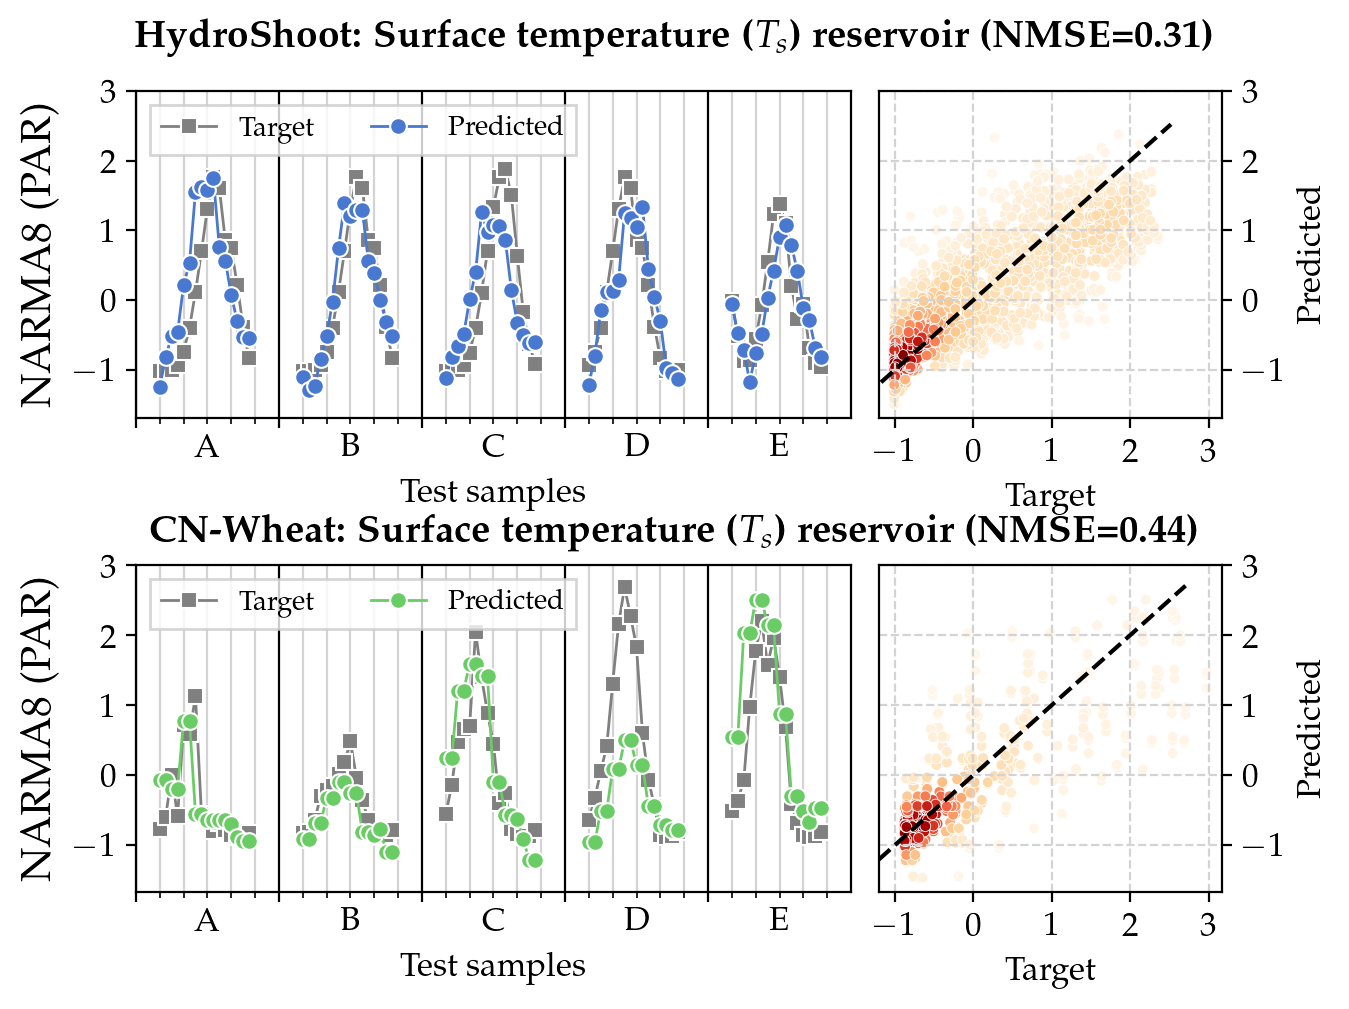
\includegraphics[width=\linewidth,height=\linewidth,keepaspectratio]{imgs/regression_res_prediction__input_PARi_NARMA_8__state__Ts_compact.png}
        \caption{\null}
        \label{fig:result-narma-accuracy}
    \end{subfigure}
    \hfill
    \begin{subfigure}[a]{0.427\linewidth}
        \centering
        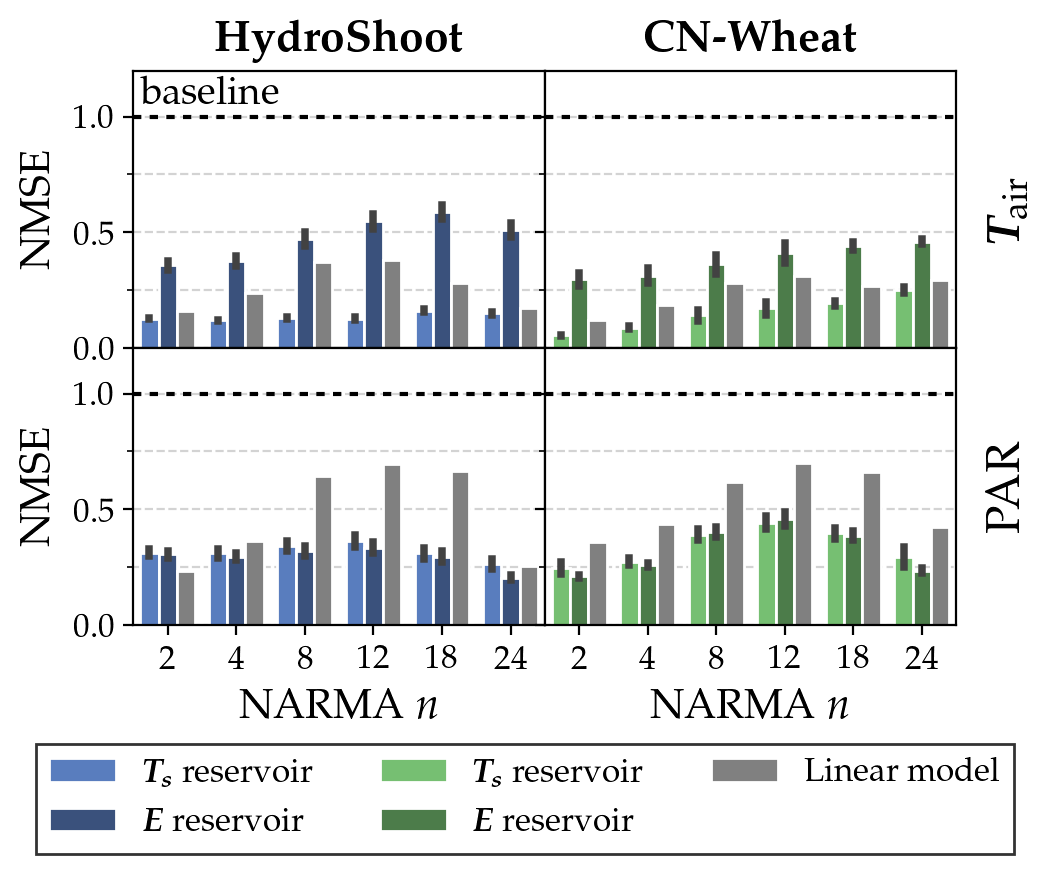
\includegraphics[width=\linewidth,height=\linewidth,keepaspectratio]{imgs/comp_NARMA_perf_compact.png}
        \caption{\null}
        \label{fig:result-narma-scores}
    \end{subfigure}
    \caption{\small
            Results for input, physiological, and computational tasks.
            Each figure shows the distribution of test scores for 16 random reservoir samplings.
            (\subref{fig:result-regression-scores}):
                Reservoir performance for input and physiological regression tasks.
                The plots show prediction accuracy for a suite of regression tasks for each of the physiological reservoirs from \mbox{Table \ref{table:simulation_reservoirs}}.
                The regression target of net photosynthesis rate  $A_n$ was only available for the HydroShoot model.
                The box shows the quartiles of the distribution; the whiskers indicate the 5th and 95th percentiles.
                % Outliers are shown as a diamond shape;
            (\subref{fig:result-delay-scores}, \subref{fig:result-polynomial-scores}, \subref{fig:result-narma-scores}):
                Predicting a delayed signal, polynomial expansion, and NARMA task based on $T_{\text{air}}$ and PAR using surface temperature ($T_s$) and transpiration rate ($E$).
                The reservoirs' performance is compared to a linear model that uses the benchmark's input as the only feature.
                The error bars show the scores' standard deviation;
            (\subref{fig:result-regression-accuracy}, \subref{fig:result-narma-accuracy}):
                Time series prediction of absorbed PAR and NARMA8 using $E$ and  $T_s$, respectively.
                The left plot shows predictions for five days randomly sampled from the test set.
                the right shows correlation between target and predicted values. Darker colors indicate a greater density of points.
        }
    \label{fig:results}
\end{figure*}


\subsection{Applications}
% Applications of reservoir computing with plants?
If plants can behave like reservoir computers, RC may become a versatile addition to the agricultural R\&D toolbox.
For example, new insights could be gained into eco-physiological processes by observing and measuring the relationship between environmental signals (reservoir input) and plant behavior (reservoir dynamics).
We suspect there are many possibilities for discovering new phenomena with this holistic data-driven approach, especially on the time scale between seconds and minutes.
In addition, reservoir computing can have applications in phenotyping. 
The RC framework may identify phenotypes that are better at integrating their environmental inputs into an adaptive response.
Especially rapid responses are currently underexplored in phenotyping research, even though they play an essential role in plant life \cite{alarcon_substantial_1994, de_swaef_plant_2015}.
Even further down the road, RC can find applications in autonomous greenhouses. RC can measure the plant's response to the conditions set by the grower or an autonomous control system in real-time. 
A closed-circuit control loop could even be designed to let the plant itself controls the delivery of light, water, and nutrients.


\section{Conclusion}

% *Conclusions from results*
Regression benchmarks show promising results for plant RC with several plant physiological processes.
In addition, the analysis of fading memory revealed chaotic behavior in physiological processes and unexpected behavior in a plant model that was previously unreported.

To select physiological reservoirs for future research, we recommend cross-referencing our results of reservoir performance with available sensing technologies.
For example, surface temperature, transpiration rate, and stomatal conductance form a good combination of reservoir features because they can be observed using thermal cameras \cite{pieters_reservoir_2022}.

% *Expanding on the foundation:*
The study of using plants as a substrate for reservoir computing is still in its infancy.
There are several yet unexplored topics to extend the foundation of plant RC.
We currently only have data on RC with three species: strawberry plants in prior work and now \textit{in silico} versions of grapevine and wheat.
Another area that requires attention is how RC can be reconciled with plant growth.

% *Moving towards applications:*
We believe that this is only the beginning of the road for plant reservoir computing.
If the knowledge and technology can scale, the opportunities in agricultural tech will be numerous.


%%%%%%%%%%%%%%%%%%%%%%%%%%%%%%%%%%%%%%%%%%%%%%%%%%%%%%%%%%%%%%%%%%%%%%%%%%%%%%%%%%%%%%%%%%


% print url if no doi
\renewbibmacro*{doi+eprint+url}{%
\printfield{doi}%
\newunit\newblock%
\iftoggle{bbx:eprint}{%
\usebibmacro{eprint}%
}{}%
\newunit\newblock%
\iffieldundef{doi}{%
\usebibmacro{url}}%
% \usebibmacro{url+urldate}}%
{}%
}


% journaltitle=false,eventtitle=false,publisher=false,booktitle=false
% \AtNextBibliography{\togglefalse{bbx:eventtitle}}
\renewcommand*{\bibfont}{\scriptsize}
\printbibliography


\end{document}

% \begin{figure}[t]
% 	\centering
%     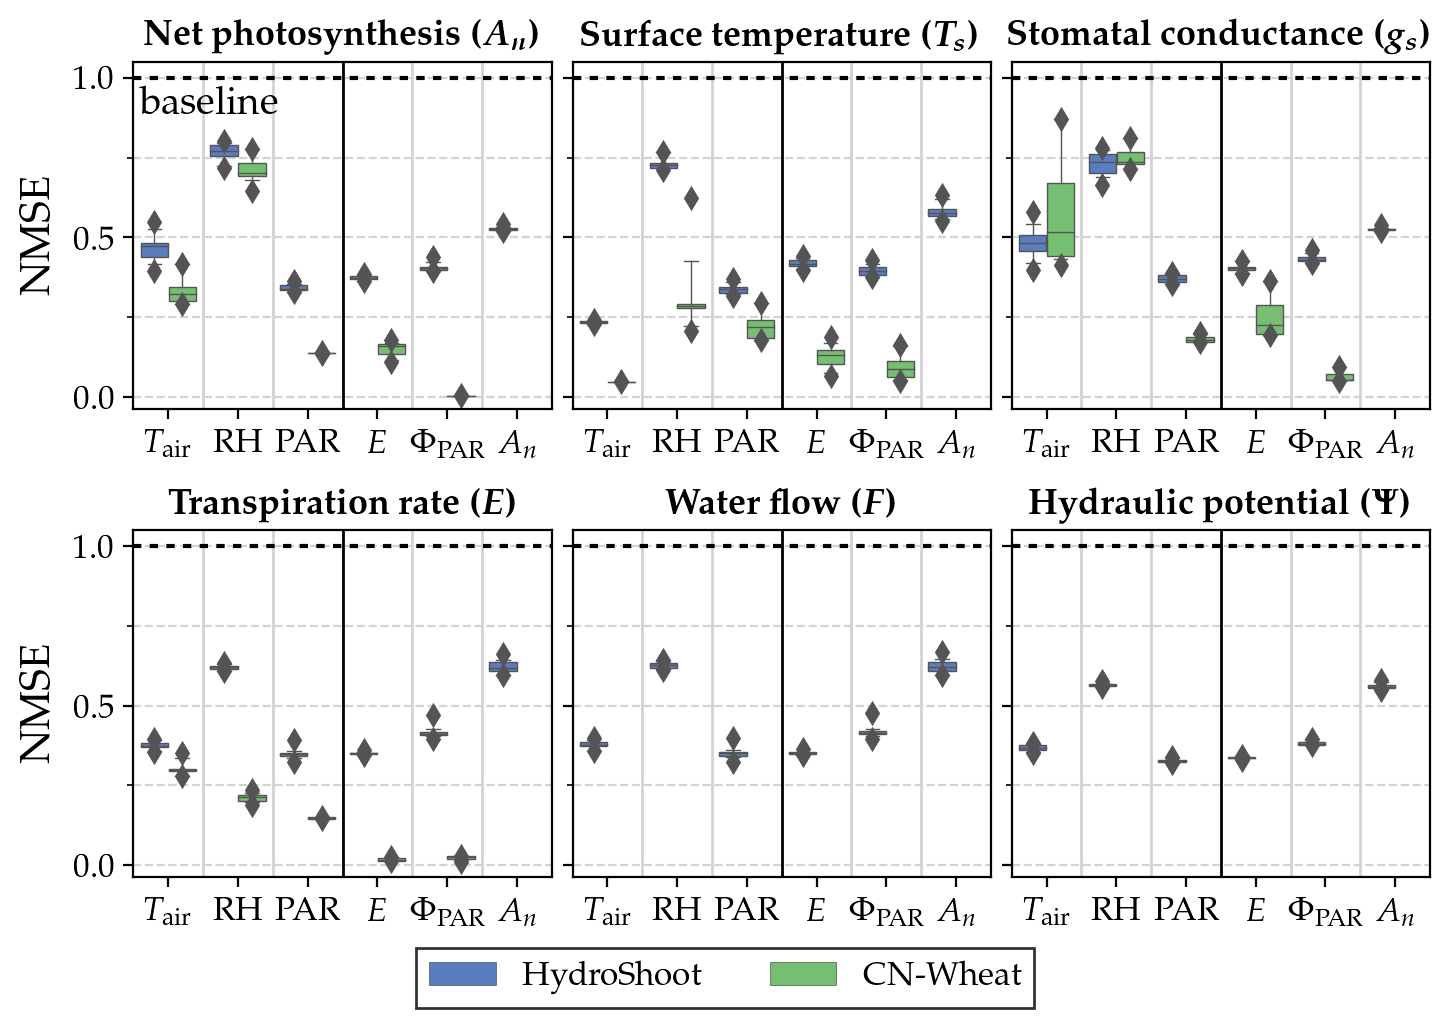
\includegraphics[width=\linewidth]{imgs/regression_res_perf_compact.png}
% 	\caption{\small
%              Reservoir performance for input and physiological regression tasks.
%              The different plots show the prediction accuracy (y axis) for a suite of regression tasks (x axis) of a physiological reservoir from \mbox{Table \ref{table:simulation_reservoirs}}.
%              The regression target of net photosynthesis rate  $A_n$ was only available for the HydroShoot model.
%              Each boxplot shows the distribution of test across 16 random reservoir samplings.
%              The box shows the quartiles of the distribution; the whiskers indicate the 5th and 95th percentiles.
%              Outliers are shown as a diamond shape.}
% 	\label{fig:input-phys-scores}
% \end{figure}


% \begin{figure}[hp]
% 	\centering
%     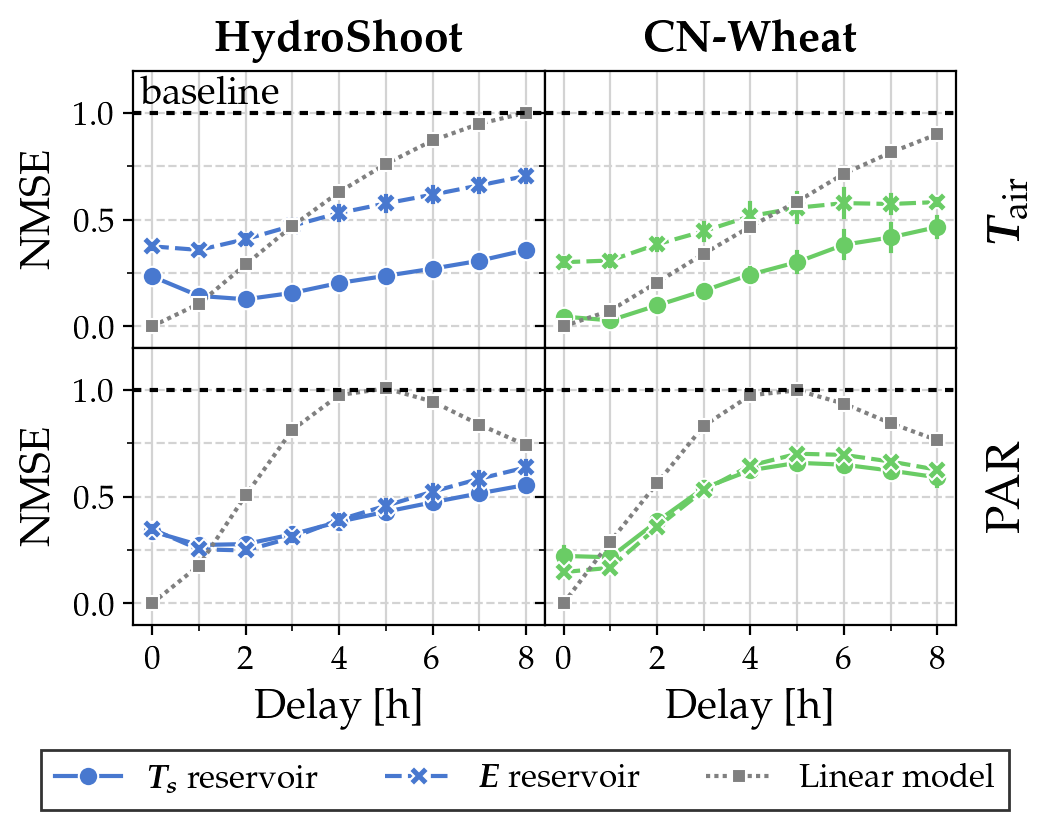
\includegraphics[width=0.85\linewidth]{imgs/comp_delay_perf_compact.png}
% 	\caption{\small 
% 	Predicting a time-delayed signal of $T_{\text{air}}$ and PAR using surface temperature ($T_s$) and transpiration rate ($E$).
%     The reservoirs' performance is compared to a linear model that uses the benchmark's input as the only feature.
%     The error bars show the scores' standard deviation.
%     }
% 	\label{fig:delay-line-scores}
% \end{figure}

% \begin{figure}[hp]
% 	\centering
%     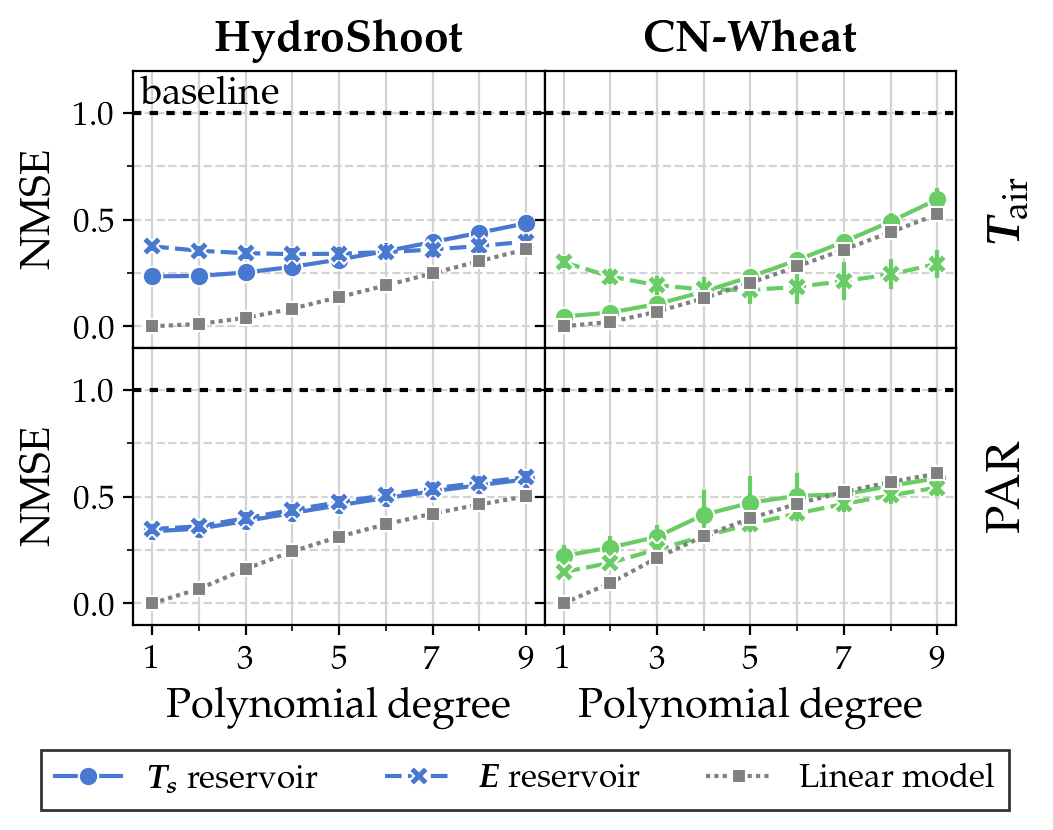
\includegraphics[width=0.85\linewidth]{imgs/comp_polynomial_perf_compact.png}
% 	\caption{\small
% 	    Predicting a polynomial expansion of $T_{\text{air}}$ and PAR using surface temperature ($T_s$) and transpiration rate ($E$).
% 	    % The reservoirs' performance is compared to a linear model that uses the benchmark's input as the only feature.
%         % The error bars show the scores' standard deviation.
%     }
% 	\label{fig:poly-task-scores}
% \end{figure}

% \begin{figure}[hp]
% 	\centering
%     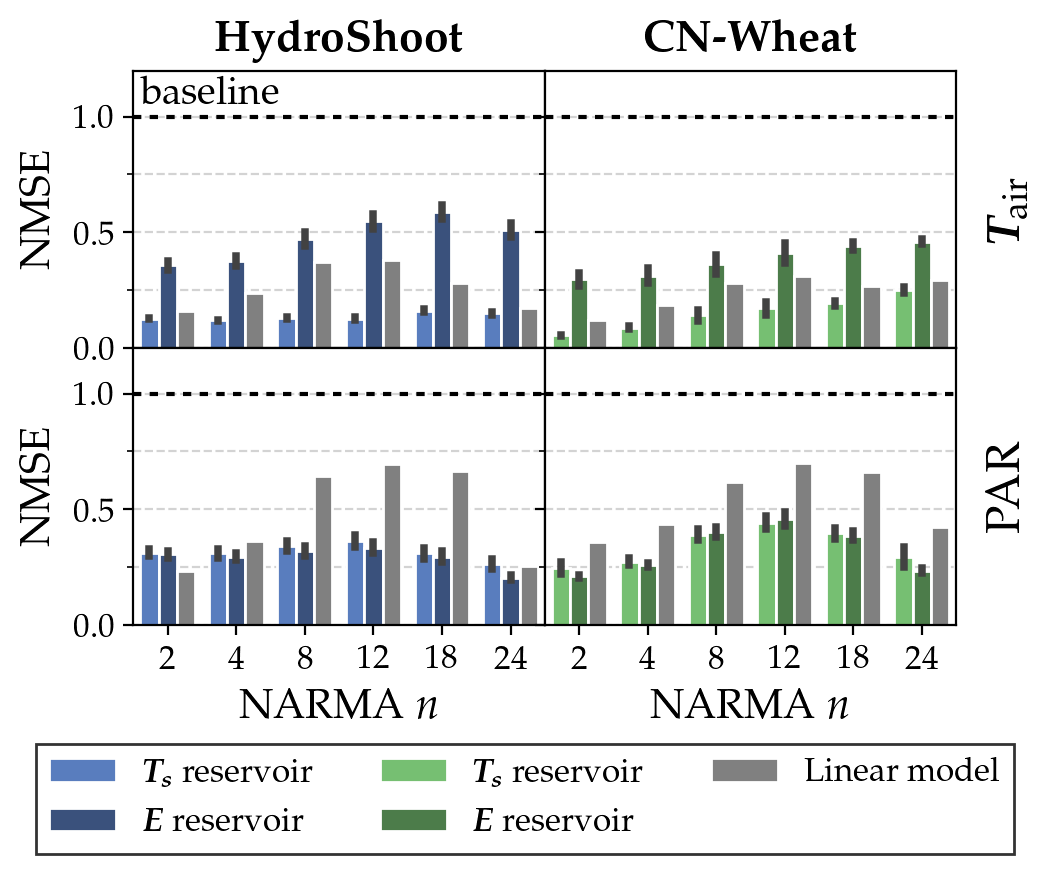
\includegraphics[width=0.85\linewidth]{imgs/comp_NARMA_perf_compact.png}
% 	\caption{\small
% 	    Predicting the NARMA benchmark based on $T_{\text{air}}$ and PAR using surface temperature ($T_s$) and transpiration rate ($E$).
% 	    % The reservoirs' performance is compared to a linear model that uses the benchmark's input as the only feature.
%         % The error bars show the scores' standard deviation.
%     }
% 	\label{fig:poly-task-scores}
% \end{figure}